\section{Introduction}

Aerodynamic Shape Optimization (ASO) is a process aimed at refining an object’s shape design to enhance its aerodynamic performance, achieving objectives such as reducing fuel consumption, increasing operating efficiency or improving maneuverability, under specified design constraints. ASO holds significant importance across various fields where it facilitates designs for applications like aerospace, automotive, and marine engineering. As shown in Fig.~\ref{ch5:fig:aso_pipeline}(a), ASO typically involves iterative cycles of computational fluid dynamics (CFD) simulations, visualization and expert analysis, shape modeling and modification, and mesh deformation or remeshing. Traditional ASO can be both slow and costly, with shape parameterization and its associated geometric processing being especially labor-intensive.

Shape parameterization is central to ASO. It provides the mathematical framework through which object geometries are represented and manipulated. Its influence on ASO performance is both profound and multifaceted. The choice of parameterization approach defines the optimization boundaries, determining the maximum geometric complexity that can be handled, the allowable range of shape modifications, and the achievable level of surface smoothness. Then a key challenge lies in balancing the dimensionality of the parameter space with optimization effectiveness: a high-dimensional parameter space enables detailed geometric modeling but may hinder convergence, while a lower-dimensional space facilitates faster optimization but can restrict the search within the design space. Furthermore, the parameterization method directly impacts ASO’s implementation costs due to the level of human intervention required: from initial surface modeling and design variable configuration to the management of CFD mesh deformation. Consequently, selecting an effective parameterization approach is critical for achieving cost-effective and efficient ASO.

Given its critical importance, shape parameterization has been the focus of extensive research. Traditional approaches include Hicks-Henne bump functions~\cite{aa.Hicks1978}, non-uniform rational B-spline (NURBS) curves, and class-shape function transformation (CST)\cite{aa.Kulfan2008} for two-dimensional applications, while free-form deformation (FFD)~\cite{aa.Sederberg1986, aa.Lamousin1994, aa.Kenway2010} is preferred for three-dimensional problems. Despite their success, these traditional methods face notable challenges. The performance and computational efficiency of ASO are highly sensitive to how the parameterization is implemented, including the choice of algorithm and hyperparameters~\cite{aa.Masters2017,aa.Vuruskan2019,aa.Song2004}, with no formal methodology to identify optimal configurations. This leads practitioners to rely on trial-and-error approaches, empirical knowledge, or adaptation of methods from similar cases, followed by extensive manual tuning. This reliance on manual processes makes traditional methods impractical for rapid prototyping and iterative design, where efficiency and adaptability are crucial. Moreover, designers must balance trade-offs between deformation freedom, optimization effectiveness, and global surface smoothness. While high-dimensional design variables provide greater design flexibility, they complicate optimization and increase the risk of poor convergence. Ensuring global surface smoothness is also challenging with large deformation freedom, where even minor surface inconsistencies can cause glitches in simulation, disrupting the optimization process.
Furthermore, traditional parameterizations solely focus on the surface geometry, necessitating separate processing of volumetric CFD meshes through deformation or re-meshing, which adds substantial implementation complexity. While AI-based parameterization models have emerged as alternatives~\cite{aa.Bamford2024,aa.Swannet2024,aa.Secchi2024}, their data-driven nature requires a large-scale training dataset and introduces new challenges on data engineering, particularly in aerospace applications where training data is scarce and computationally expensive to generate. The geometric priors learned by these models are inherently limited by the dataset available, making any newly generated shape an interpolation of existing data rather than a truly novel design. Consequently, AI-based models lack the innovation potential of free-form parameterization methods, which offer greater design space exploration.

To address these limitations, we aim at building an AI-assisted ASO pipeline and introduce the Deep Geometric Mapping (DeepGeo) model, a novel neural network-based approach that unifies shape representation and mesh deformation within a single framework, as shown in Fig.~\ref{ch5:fig:aso_pipeline}(b). DeepGeo uses a Multi-Layer Perceptron (MLP) to parameterize both the surface geometry and the surrounding CFD computational volumetric mesh, the latter being necessary for aerodynamic performance evaluation through CFD simulations. 
As illustrated in Fig.\ref{ch5:fig:pipeline}(a), DeepGeo's initialization phase involves training the MLP to deform the surface vertices from a template shape to align with the target geometry, the starting configuration for optimization.
The surrounding volumetric mesh is simultaneously deformed to ensure consistency with the surface geometry. By accurately reconstructing the target geometry, this initialization process encodes the geometric information within the network weights. 
Shape optimization is then performed by applying an adjoint-based method~\cite{aa.Jameson1995} to minimize aerodynamic objective functions and enforce geometric constraints with respect to these weights, as shown in Fig.\ref{ch5:fig:pipeline}(b). 
The updated weights enable DeepGeo to output a CFD mesh that defines a new geometry, thus manipulating the shape design iteratively. The optimization process continues until convergence is reached.
This formulation establishes the network weights as the parameterization for both the surface shape and the volumetric mesh, enabling automated regeneration of the necessary CFD mesh as the geometry evolves with every optimization iteration. By unifying shape parameterization and mesh deformation within a single framework, DeepGeo significantly reduces traditional ASO implementation complexities and streamlines the optimization pipeline, by removing the need for a separate CFD mesh deformation or remeshing module and the associated time-consuming manual hyperparameter tuning. This simplification accelerates the ASO process.

% !TEX root = ../main.tex
% !TEX spellcheck = en-US

\begin{figure}[tbh]
    \begin{center}
        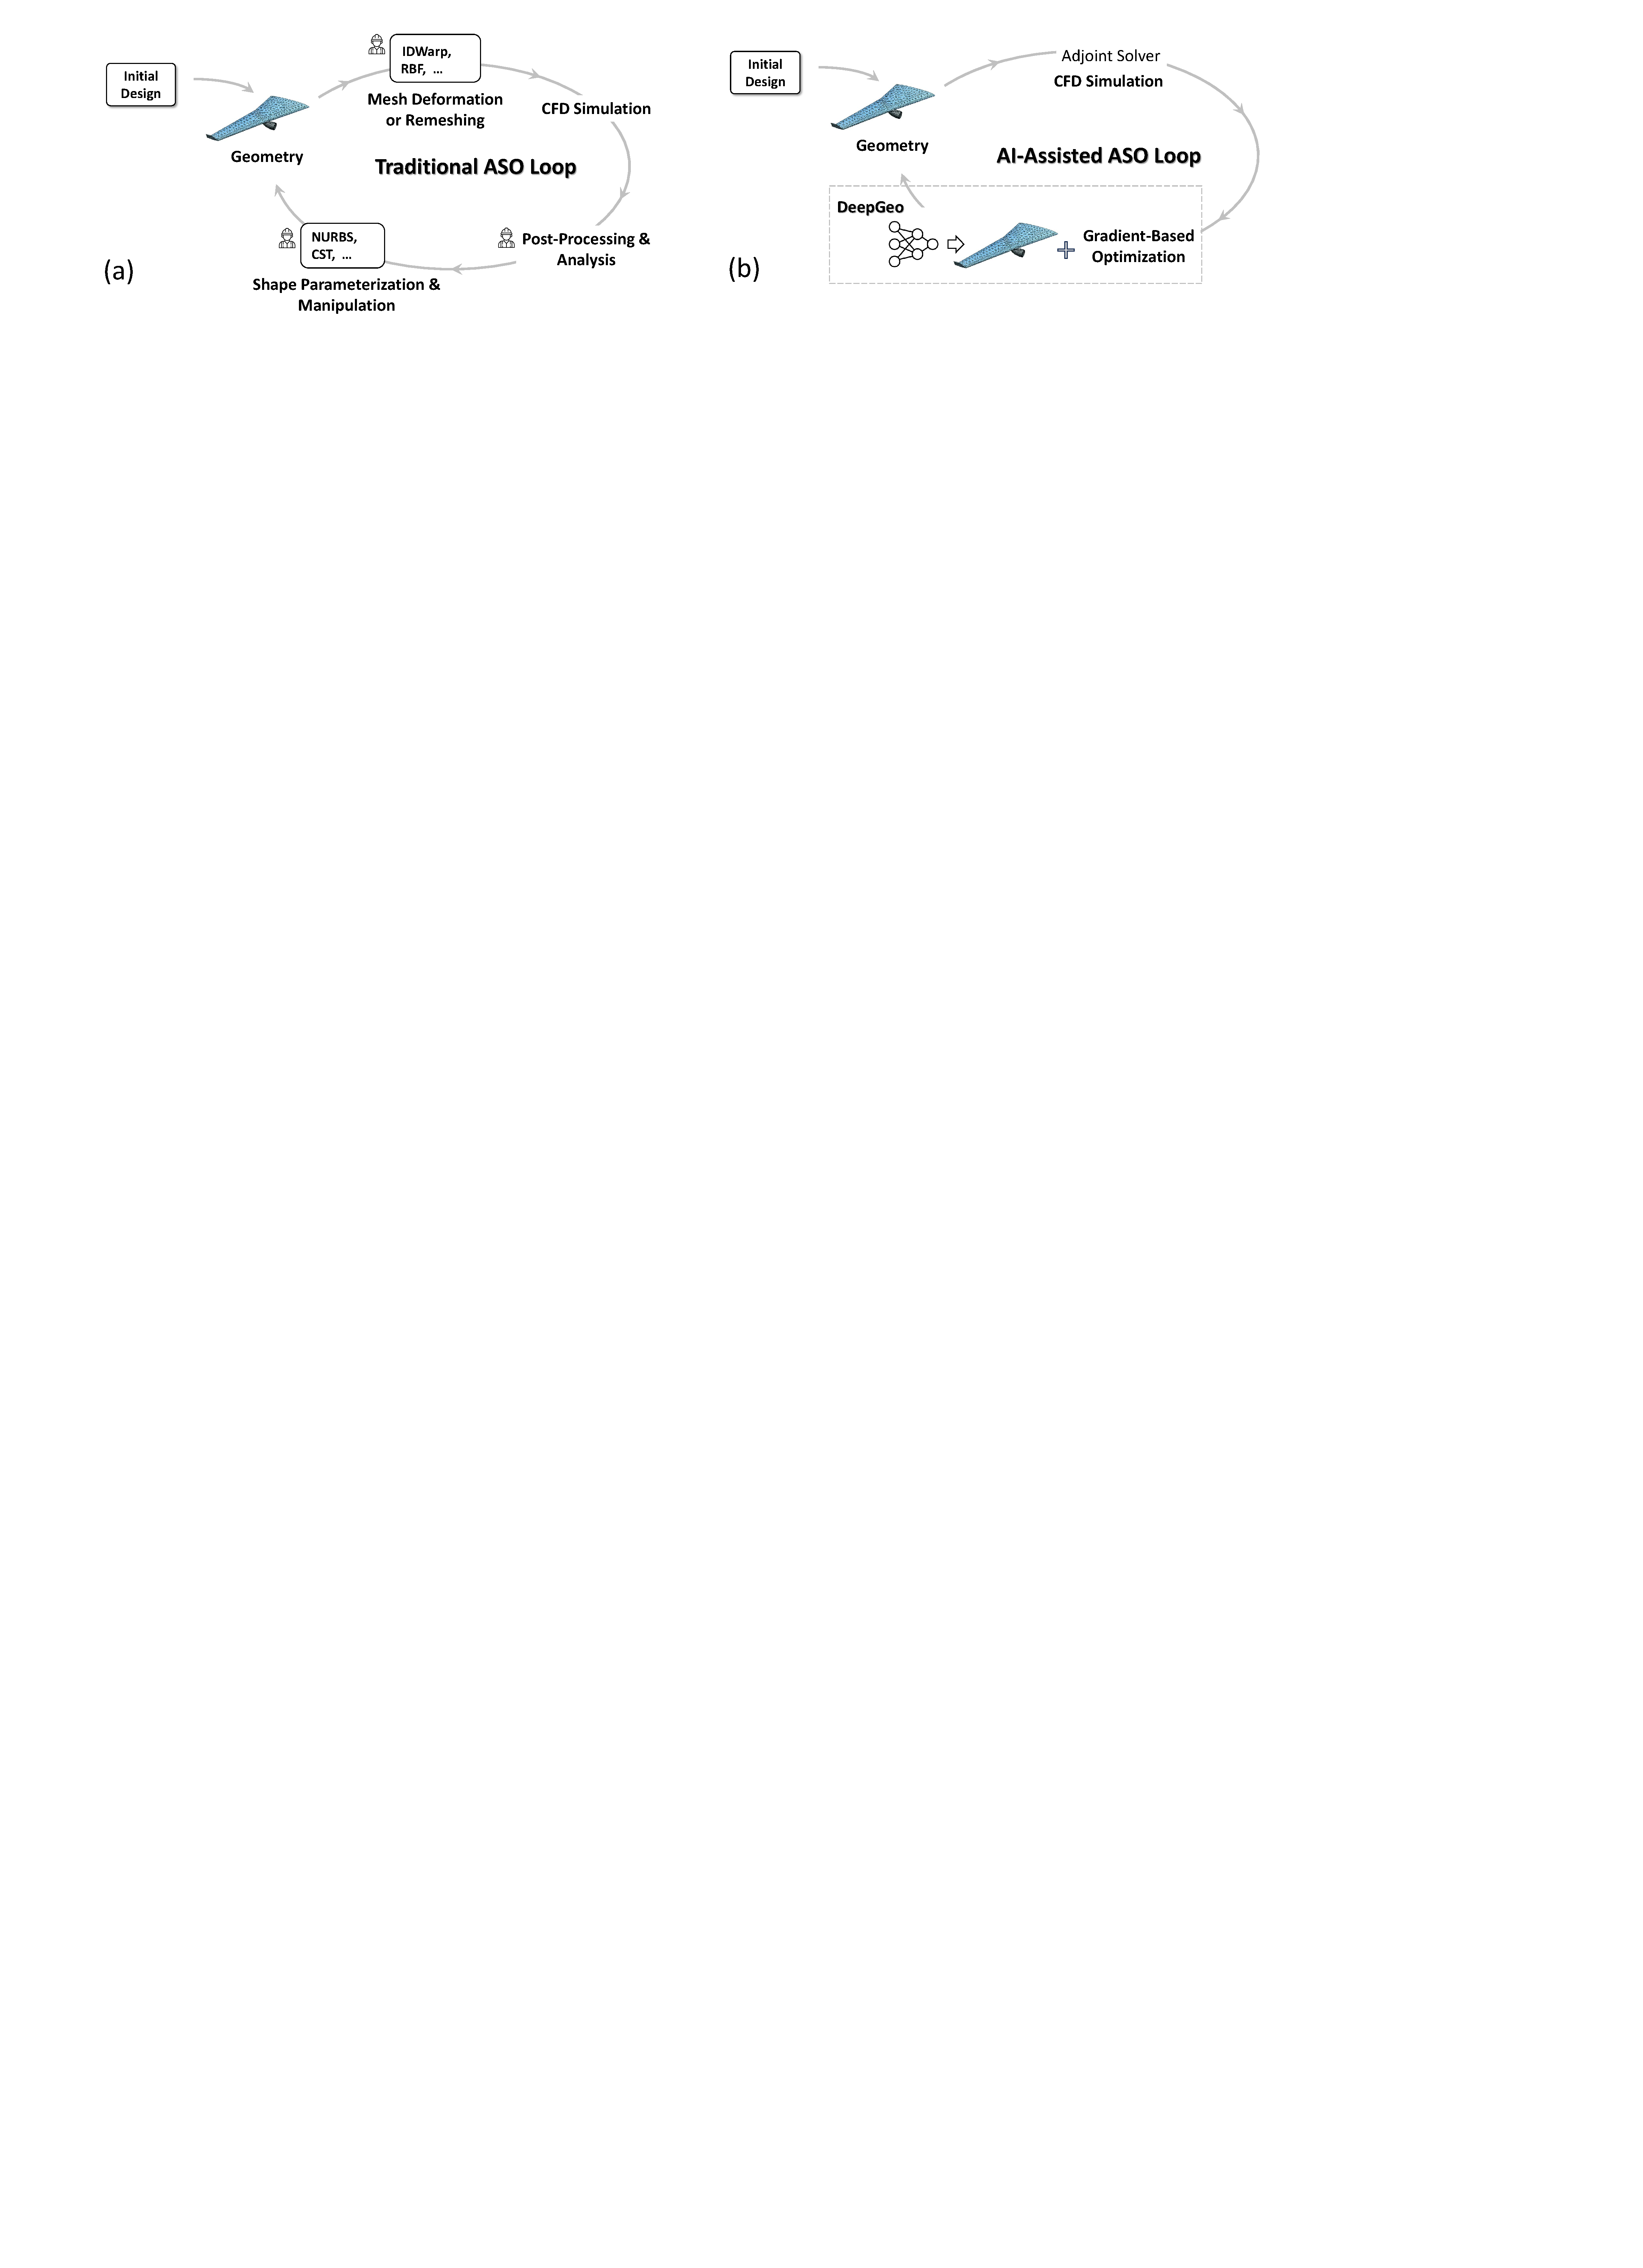
\includegraphics[width=1\linewidth]{chapter5/fig/aso_pipeline.pdf}
    \end{center}
    \vspace{-3mm}
    \caption{
        \small The pipelines of (a) traditional ASO and (b) ASO that employs DeepGeo.
    }
    \label{ch5:fig:aso_pipeline}
\end{figure}
% !TEX root = ../main.tex
% !TEX spellcheck = en-US

\begin{figure}[tbh]
    \begin{center}
        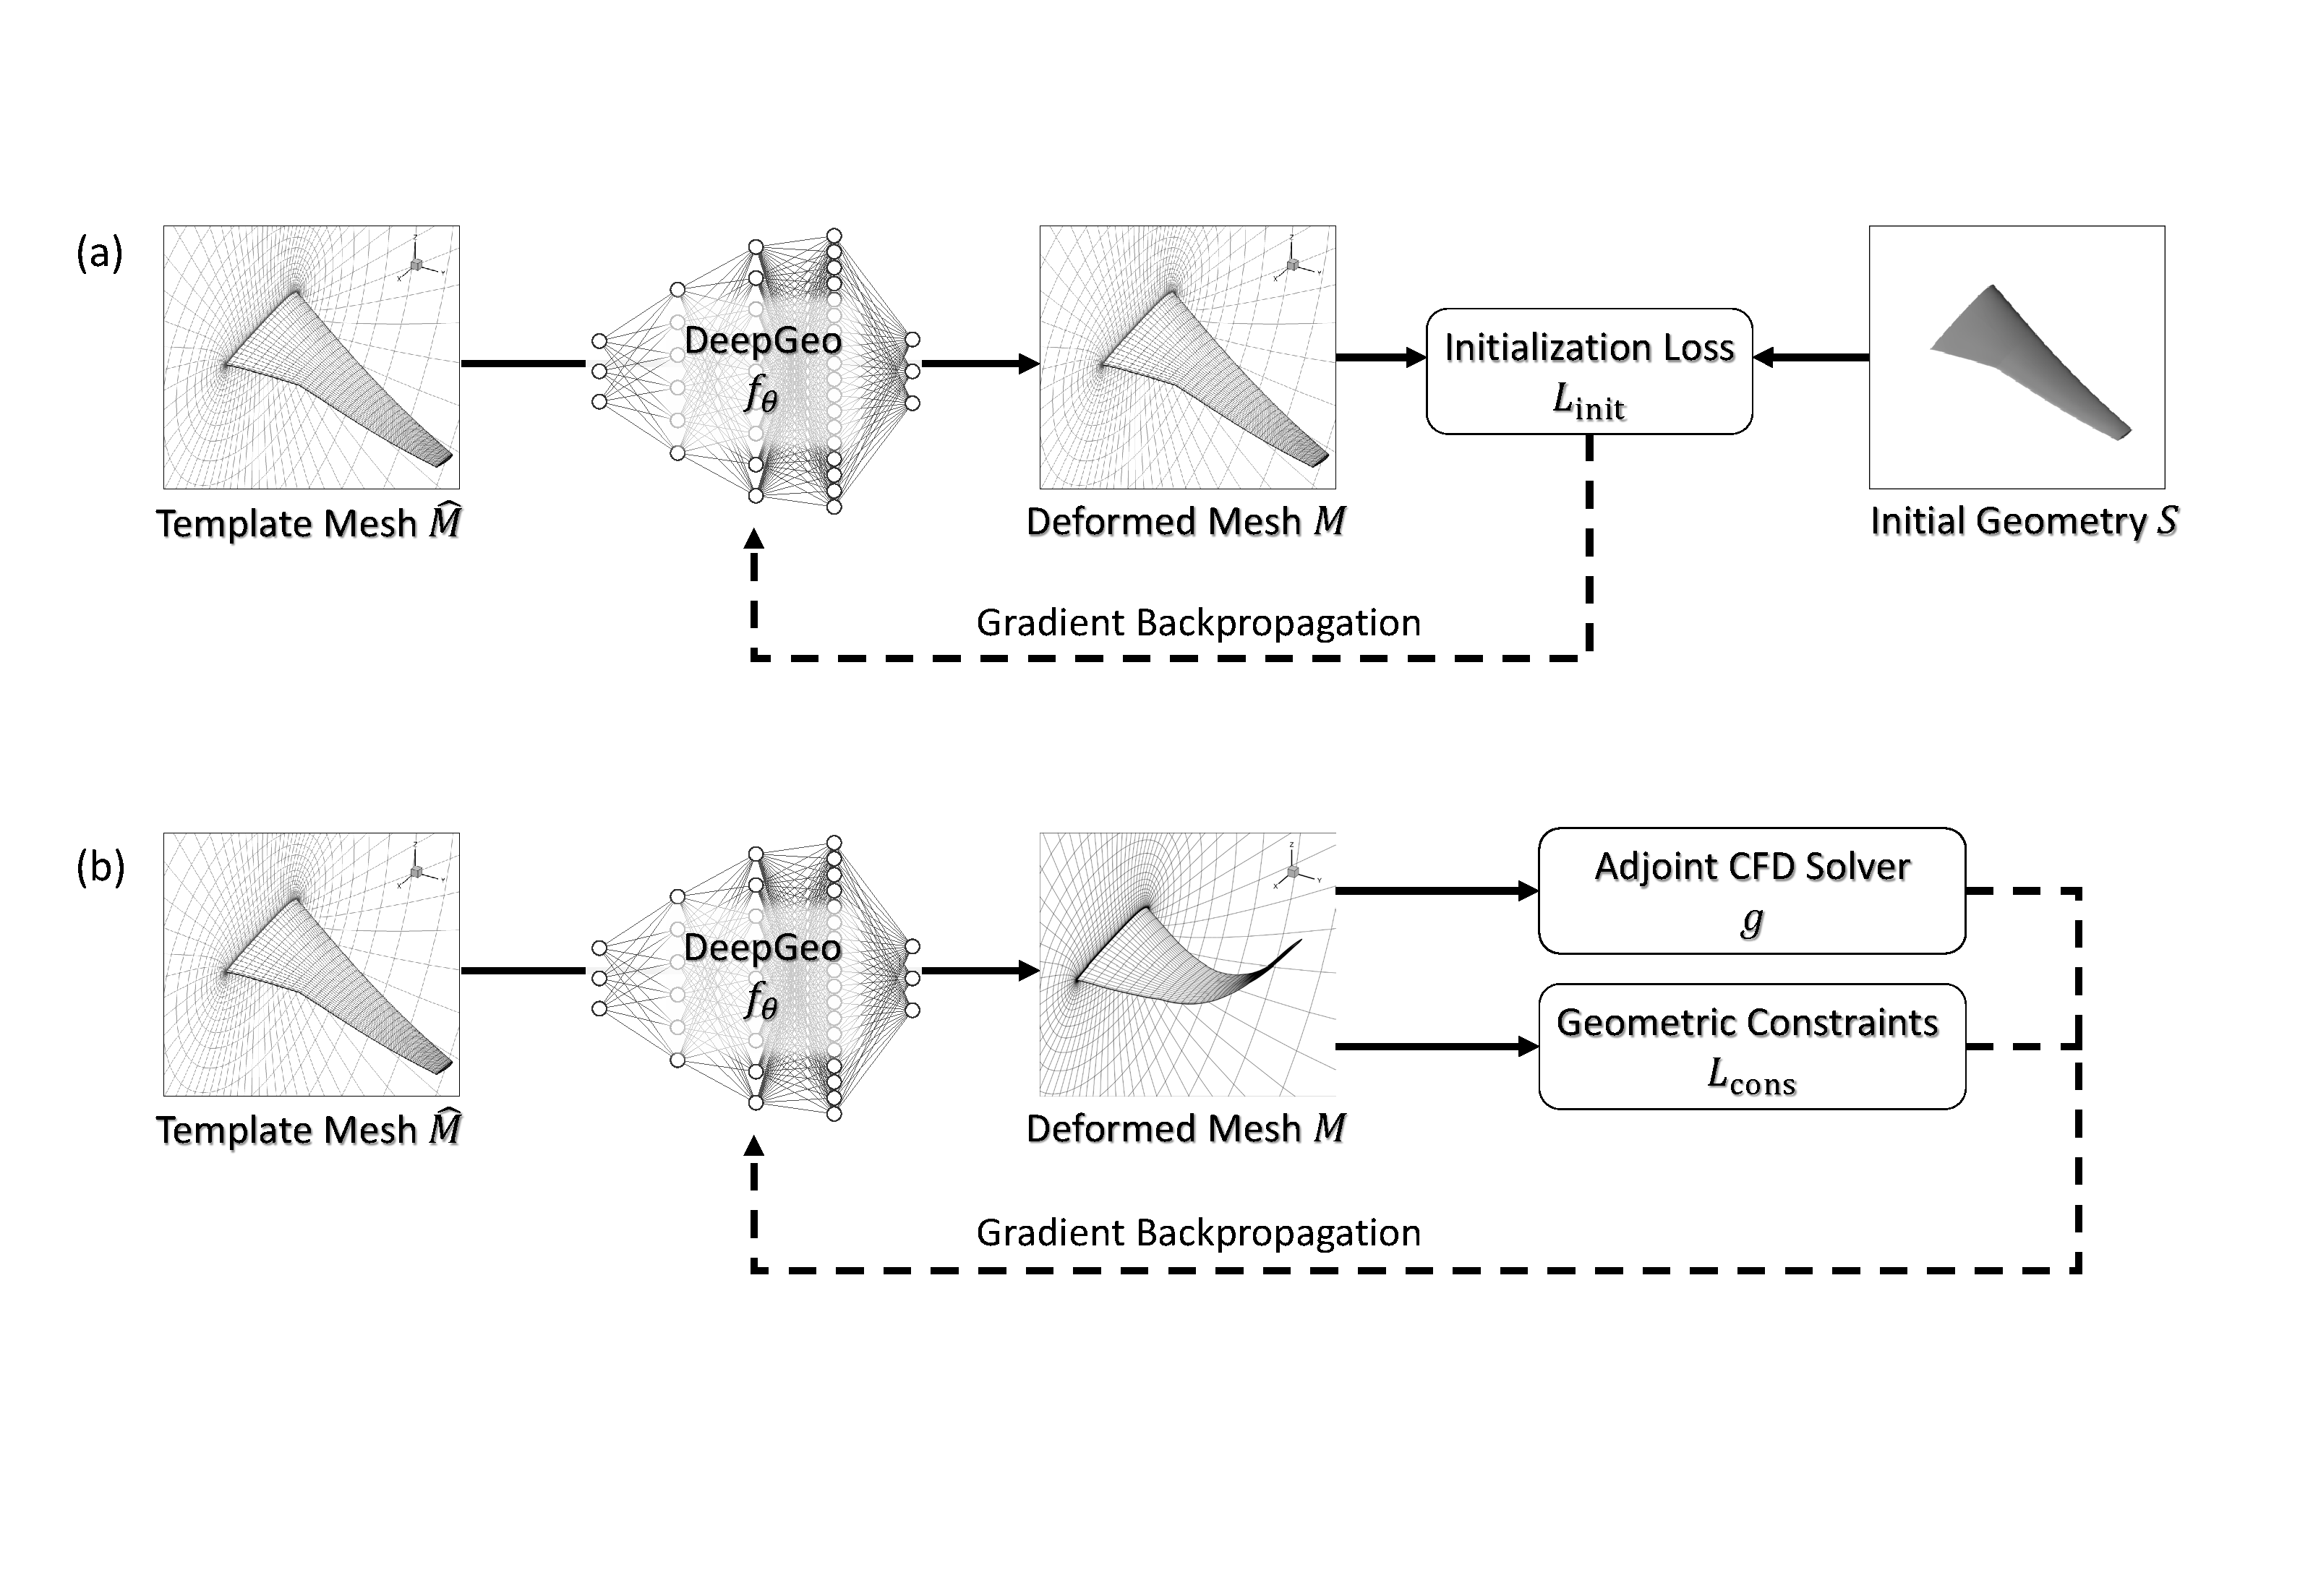
\includegraphics[width=1\linewidth]{chapter5/fig/pipeline.pdf}
    \end{center}
    \vspace{-3mm}
    \caption{
        \small The pipeline that employs DeepGeo in ASO, including (a) the initialization and (b) shape optimization stages.
    }
    \label{ch5:fig:pipeline}
\end{figure}
\begin{figure}[!htb]
    \begin{center}
        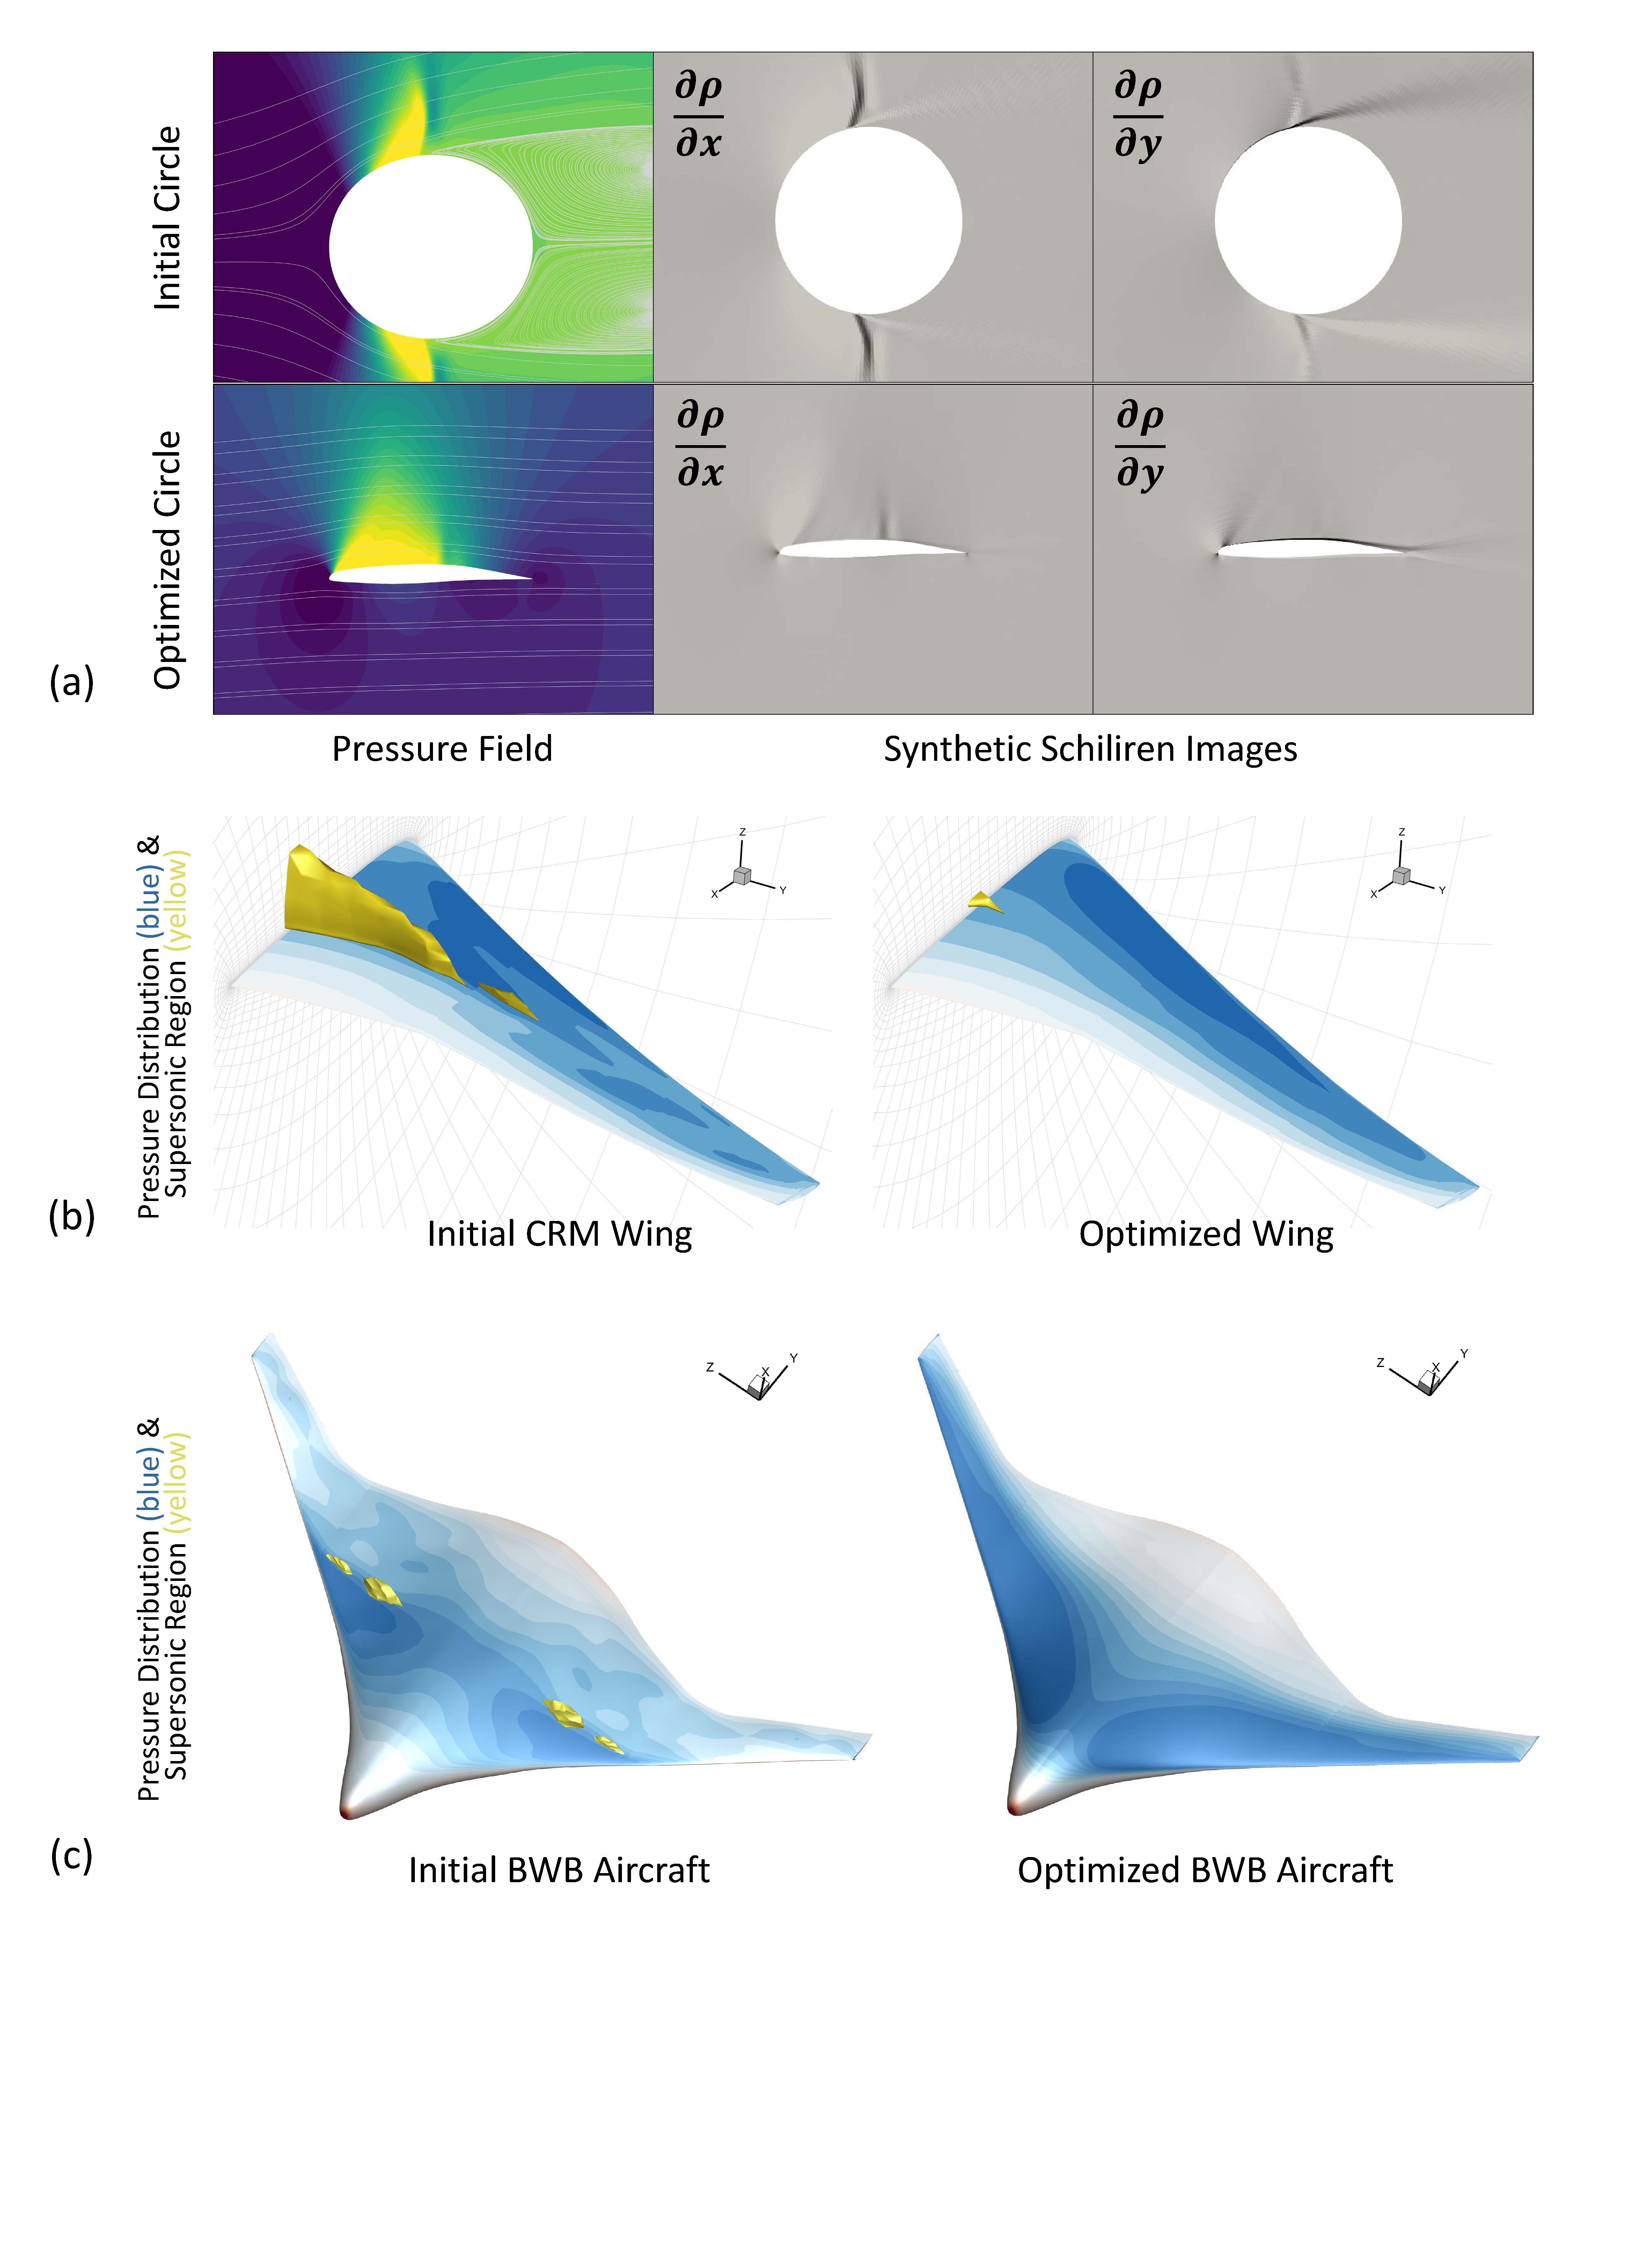
\includegraphics[width=0.9\linewidth]{chapter5/fig/teaser.pdf}
    \end{center}
    \vspace{-3mm}
    \caption{
        \small The three ASO case studies implemented by DeepGeo, including optimization from (a) 2D circle, (b) CRM wing and (c) BWB aircraft.
    }
    \label{ch5:fig:teaser}
\end{figure}

DeepGeo leverages the expressive capacity of MLPs, which comes from their ability to represent complex nonlinear mappings as layered compositions of simple functions. Thus, DeepGeo can capture rich geometric transformations and handle large deformations, while maintaining global surface smoothness. This expressiveness is key to achieving smooth, continuous transformations across complex geometries, a critical ability in high-fidelity shape optimization. DeepGeo's MLP backbone makes it possible to explore high-dimensional design spaces using a gradient-based approach by mitigating the curse of dimensionality or issues with over-parameterization~\cite{ai.Barron1993,ai.Poggio2017}. DeepGeo directly addresses the dimensionality challenges that limit traditional optimization methods, such as CMAES~\cite{ai.Hansen2016}, which become impractical beyond approximately 100 design parameters. 
Furthermore, DeepGeo’s initialization requires only a target shape and a single template mesh to set its initial weights, in contrast to data-driven approaches that rely on extensive training datasets. This minimal data requirement significantly reduces implementation complexity, decreasing dependency on large datasets and making DeepGeo especially suitable for practical aerospace applications where geometric data is often scarce.

In earlier work~\cite{aa.Wei2023b}, we introduced the Direct Mapping Model, an initial version of DeepGeo developed to handle 2D airfoil optimization. In this paper, we extend the model to address more complex optimization tasks and 3D shapes, including 2D circle optimization, 3D wing optimization, and the optimization of a 3D Blended-Wing-Body aircraft. DeepGeo achieves optimization results comparable with the state-of-the-arts, without any case-specific adaptation and requiring training dataset, as shown in Fig.~\ref{ch5:fig:teaser}.